\section{System Architecture}

\subsection{Architectural Overview}
The "Trade Helper" application is architected as a cloud-native, serverless web application. This design choice ensures high availability, automatic scalability, and low operational costs—key factors for a tool targeting retail investors. The system comprises three main layers: the Presentation Layer (Client), the Application Layer (Serverless API), and the Data Layer (External APIs).

\begin{figure}[H]
    \centering
    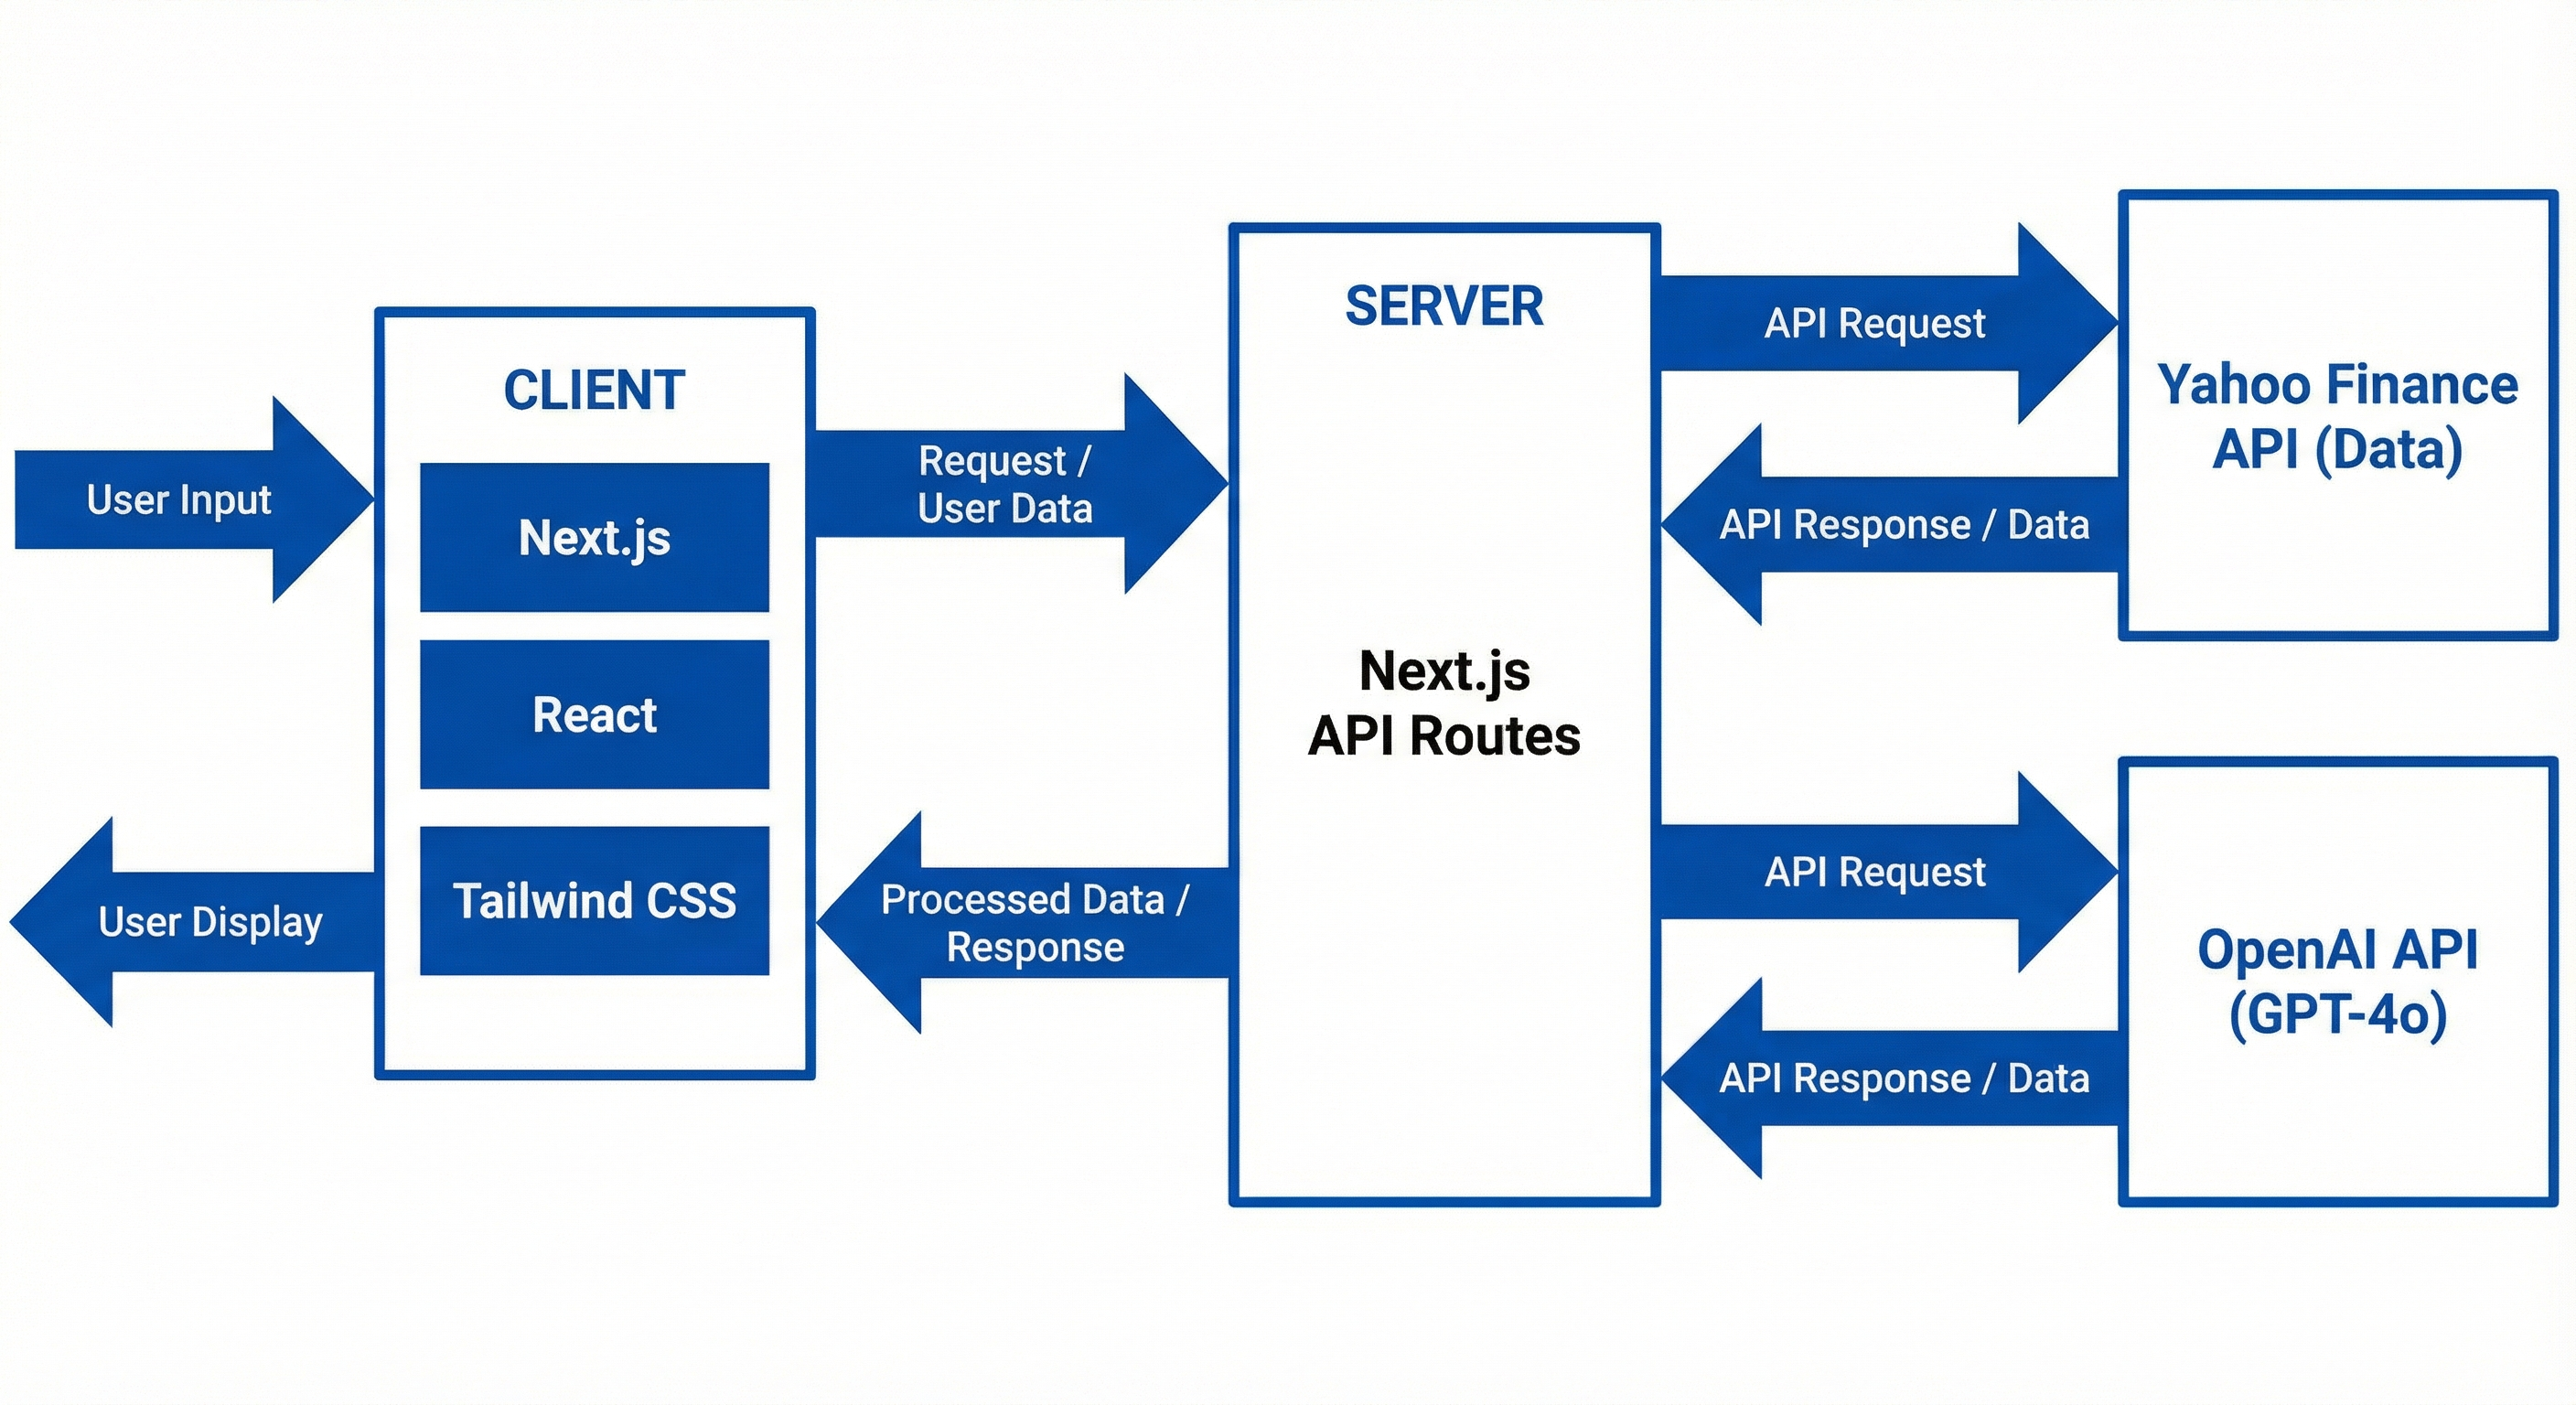
\includegraphics[width=1.0\textwidth]{images/architecture_diagram.jpeg}
    \caption{Detailed System Architecture Diagram showing the data flow between the Next.js client, API routes, and external services.}
    \label{fig:architecture}
\end{figure}

\subsection{Frontend Implementation (Next.js)}
The frontend is built using Next.js 14, leveraging the React framework.
\subsubsection{Server-Side Rendering (SSR)}
We utilize Next.js's SSR capabilities to pre-render the initial state of the application. This improves First Contentful Paint (FCP) times and ensures that the application is SEO-friendly.
\subsubsection{State Management}
React's `useState` and `useEffect` hooks manage the application state. When a user searches for a stock, the state transitions through `isLoading` $\rightarrow$ `data` or `error`. This deterministic state machine prevents UI inconsistencies.
\subsubsection{Component Library}
The UI is constructed using atomic components styled with Tailwind CSS.
\begin{itemize}
    \item \texttt{StockInput.tsx}: Handles user input with debouncing to prevent excessive API calls.
    \item \texttt{StockChart.tsx}: Renders interactive SVG charts using the Recharts library.
    \item \texttt{AnalysisResult.tsx}: Displays the AI's recommendation with color-coded badges (Green for Buy, Red for Sell, Gray for Hold).
\end{itemize}

\subsection{Backend API Layer}
The backend logic is encapsulated in Next.js API Routes, which are deployed as AWS Lambda functions (or Vercel Serverless Functions).
\subsubsection{API Route: /api/finance}
This endpoint acts as a proxy to the Yahoo Finance API.
\begin{itemize}
    \item \textbf{Purpose}: To bypass Cross-Origin Resource Sharing (CORS) restrictions enforced by browsers and to hide upstream API keys.
    \item \textbf{Caching}: We implement `Cache-Control` headers (stale-while-revalidate) to cache stock data for 60 seconds, reducing latency for frequently requested stocks.
\end{itemize}

\subsubsection{API Route: /api/analyze}
This is the core intelligence engine.
\begin{itemize}
    \item \textbf{Input}: Stock Symbol, Historical Data JSON.
    \item \textbf{Process}:
        \begin{enumerate}
            \item Validates input schema (Zod library).
            \item Truncates history to the last 30 entries to fit within the context window and minimize token costs.
            \item Constructs the prompt string.
            \item Calls OpenAI API (`chat.completions.create`).
        \end{enumerate}
    \item \textbf{Output}: Parsed JSON recommendation.
\end{itemize}

\subsection{Security Considerations}
\subsubsection{API Key Management}
The OpenAI API key is stored in environment variables (`.env.local`) and accessed only on the server-side. It is never exposed to the client bundle.
\subsubsection{Rate Limiting}
To prevent abuse and control costs, we implement a token bucket rate limiter using Upstash Redis. Each IP address is limited to 10 analysis requests per minute.
\subsubsection{Input Sanitization}
All user inputs (stock symbols) are sanitized to prevent Injection attacks, although the risk is low given the nature of the data.

\subsection{Scalability and Cost Analysis}
\subsubsection{Serverless Scalability}
The serverless architecture allows the application to handle sudden spikes in traffic (e.g., during market opening hours) without manual intervention. New instances of the API functions are spun up automatically.
\subsubsection{Cost Estimation}
Using the GPT-4o model:
\begin{itemize}
    \item \textbf{Input Tokens}: ~500 tokens per request (30 days of OHLC data + instructions).
    \item \textbf{Output Tokens}: ~100 tokens per request (Recommendation + Explanation).
    \item \textbf{Cost per Request}: Approximately \$0.005.
\end{itemize}
This low cost-per-query makes the "freemium" business model viable for this application.
